\documentclass[11pt,a4paper,titlepage]{article}
\usepackage[czech]{babel}
\usepackage[T1]{fontenc}
\usepackage[utf8]{inputenc}
\usepackage[left=2cm,text={17cm,24cm},top=3cm]{geometry}
\usepackage{times}  %font
\usepackage[ruled,czech,linesnumbered,longend,noline]{algorithm2e}
\usepackage{algorithmic}
\usepackage{graphics}
\usepackage{picture}
\usepackage{lscape}
\usepackage{graphicx}
\usepackage{booktabs}
\usepackage{circuitikz}
\usepackage{caption}
\usepackage{pgfplots}
\usepackage{pgfplotstable}
\usepackage{array}
\usepackage{colortbl}

\pgfplotstableset{% global config, for example in the preamble
  every head row/.style={before row=\toprule,after row=\midrule},
  every last row/.style={after row=\bottomrule},
  fixed,precision=2,
}

\begin{document}

\begin{titlepage}
                    %%%%%%%%%---TITLE PAGE---%%%%%%%%
\begin{center}
                      
{\Huge\textsc{ Vysoké učení technické v Brně }}\\
\bigskip
{\LARGE\textsc{ Fakulta informačních technologií }}\\
\bigskip
\vspace{\stretch{0.382}}
{\LARGE{Elektronika pro informační technologie}\\
\medskip
\textbf{\Huge Laboratoř č. 2}}
\vspace{\stretch{0.618}}

\end{center}
{\Large\today \hfill Vít Janeček }
\end{titlepage}
    

\section{Zadání}
Cílem této laboratoře bylo podle schématu postavit obvod pro měření VA charakteristiky,
změřit VA charakteristiku diody a výsledné hodnoty zapsat do tabulky.
Dále pak do grafu VA charakteristiky vyznačit pracovní bod.
\section{Teorie}

VA charakteristika - zobrazení vyjadřujíjí závislost mezi proudem procházející součástkou a napětím na součástce \\
Nelineárlní součástka - součástka, která nemá lineární VA charakteristiku \\
Pracovní Bod - bod VA charakteristiky, kteý odpovídá zapojení součástky v určitém obvodu za klidovího stavu\\
Potenciometr - součástka s třemi vodiči, která umí plynule rozdělit odpor.
Potenciometr připojen krajními vodiči má odpor R. Prostřední vodič rozděluje R na $R_{1}$ a $R_{2}$, které jsou tak s prostředním vodičem zapojeny do hvězdy.
Poměr lze měnit, ale vždy platí $R_{1} + R_{2} = R$.
Pokud zapojíme zbytek obvodu mezi krajní a střední vodič, pak můžem plynule ovládat napětí v tomto obvodu (teoreticky od 0 až po napětí baterky).

           
\section{Měření}

Měření jsem bylo provedeno podle následujícího schématu. Odpor $R_{S}$ bylo nutné přidat, jinak by mohlo dojít k poškození diody.
V obvodu nalevo od měření $U_{0}$ je všude shodný proud.
Měření konkrétních hodnot pro stejné $U_{0}$ bylo zapsáno co nejrychleji za sebou, aby se omezily nepřesnosti.

\begin{center}
    \begin{circuitikz}[line width = 0.8pt, voltage shift = 0.7, scale=1,transform shape]
        \draw
        (1,1) to (4,1) to (4,1) to [short, -*] (5,1) to[ammeter, l=$I_{N}$]  (9,1) to [thermistor] node[xshift=-15pt,yshift=-20]{$R_{N}$}(9,3) to [european resistor, -*] node[xshift=35,yshift=0]{$R_{S}$} (5,3) to (3.5,2.26)
        (3,4) to (1,4) to [american voltage source, n=u1] (1,1)
        (3,1) to [tgeneric, l=$R_{pot}$] (3,4)
        (5,3) to [open,v=$U_{0}$]node[xshift=15pt,yshift=70,left]{$5V$} (5,1)
        (9,2.8) -- (10,2.8) to[voltmeter, l=$U_{N}$] (10,1.2) -- (9,1.2)
        (6,3) -- (6,4) to[voltmeter, l=$U_{S}$] (8,4) -- (8,3)
    \end{circuitikz}
\end{center}



\begin{table}[h]
    \begin{center}
        \begin{tabular}{|c|c|c|c|c|c|c|c|c|c|c|}\hline
        $U_{0}$ & 0 & 0.2 & 0.4 & 0.6 & 1 & 2& 3 & 4 & 5 & [V] \\ \hline
        $U_{N}$ & 0 & 0.2 & 0.4 & 0.43 & 0.47 & 0.52 & 0.54 & 0.56 & 0.59 & [V] \\ \hline
        $I_{N}$ & 0 & 0.4 & 6 & 31 & 84 & 214 & 346 & 541 & 874 & [µA] \\ \hline
        $U_{SN}$ & 0 & 0.2 & 0.36 & 0.58 & 0.87 & 1.52 & 2.15 & 3.06 & 4.53 & [V] \\ \hline
        $I_{K}$ & 0 & 43 & 86 & 129 & 215 & 430 & 645 & 860 &  1075 & [µA] \\ \hline
        \end{tabular}
    \end{center}
\end{table}

\begin{center}
    Hodnoty $I_{k}$ byly spočteny podle ohmova zákona z  $U_{0}$ a $R_{S} = 4.65k\Omega$
\end{center}

\begin{center}
    \begin{figure}[h]
            \centering
            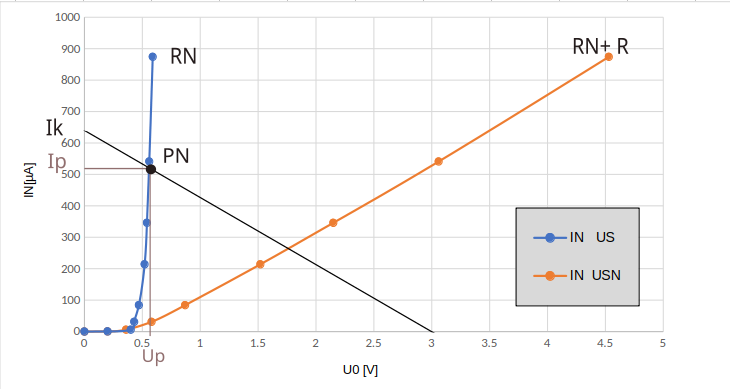
\includegraphics[width=0.7\textwidth]{./graf_Image}
            \captionsetup{labelformat=empty}
            \caption{VA charakteristika, nalezený pracovný bod diody  $P_{N}$ pro $U_{0} = 3V$ a $I_{k} = 645 \mu A$}
    \end{figure}
\end{center}
 \\ \\\ \\ \\
\section{Závěr}
VA charakteristka součásky označuje jaký proud součástkami protéká při různých proudech.
Pomocí potenciometru můžeme změřit rozsah mezi nulou a napětím baterie.
Dioda v závislosti na proudu a napětí mění svůj odpor a tak její VA charakteristika není lineární.


\end{document}
